%%%%%%%%%%%%%%%%%%%%%%%%%%%%%%%%%%%%%%%%%%%%%%%%%%%%%%%%%%%%%%%%%%%%%%%%%%%%%%%%
% Preámbulo                                                                    %
%%%%%%%%%%%%%%%%%%%%%%%%%%%%%%%%%%%%%%%%%%%%%%%%%%%%%%%%%%%%%%%%%%%%%%%%%%%%%%%%

\documentclass[11pt,a4paper,titlepage,oneside]{report}

%%% RELACIÓN DE VARIABLES A PERSONALIZAR %%%
\def\lingua{gal}
%\def\lingua{esp} % descomenta esta liña se redactarás a memoria en español
%\def\lingua{eng} % descomenta esta liña se redactarás a memoria en inglés
\def\nome{Hugo Mato Cancela}                             % substitúe aquí o teu nome
\def\nomedirectorA{Roberto Rodríguez Osorio}              % substitúe aquí o nome de quen dirixe
%\def\nomedirectorB{Outro Nome Completo}             % duplica esta liña máis veces se o precisas, cambiando
                                                     % a letra final (A, B, C, D...): úsanse na portada.tex
\def\titulo{Simulador de RISC-V empregando SystemC} % substitúe aquí o título do teu TFG
%\def\titulacion{gced}                               % descomenta esta liña e comenta a seguinte se es estudante do GCED
\def\titulacion{gei}
%\def\mencion{COMPUTACIÓN}                           % descomenta a mención que che corresponda se es estudante do GEI
%\def\mencion{ENXEÑARÍA DO SOFTWARE}
\def\mencion{ENXEÑARÍA DE COMPUTADORES}
%\def\mencion{SISTEMAS DE INFORMACIÓN}
%\def\mencion{TECNOLOXÍAS DA INFORMACIÓN}

%\def\renomearcadros{si} % descomenta esta liña se redactas a memoria en español e prefires que
                         % os "cuadros" e o "índice de cuadros" se renomeen
                         % a "tablas" e "índice de tablas" respectivamente

\usepackage{estilo_tfg}

% Lista de paquetes potencialmente interesantes (uso baixo demanda)

% \usepackage{alltt}       % proporciona o entorno alltt, semellante a verbatim pero que respecta comandos
% \usepackage{enumitem}    % permite personalizar os entornos de lista
% \usepackage{eurofont}    % proporciona o comando \euro
% \usepackage{float}       % permite máis opcións para controlar obxectos flotantes (táboas, figuras)
% \usepackage{hhline}      % permite personalizar as liñas horizontais en arrays e táboas
  \usepackage{longtable}   % permite construir táboas que ocupan máis dunha páxina
% \usepackage{lscape}      % permite colocar partes do documento en orientación apaisada
% \usepackage{moreverb}    % permite personalizar o entorno verbatim
% \usepackage{multirow}    % permite crear celdas que ocupan varias filas da mesma táboa
% \usepackage{pdfpages}    % permite insertar ficheiros en PDF no documento
% \usepackage{rotating}    % permite diferentes tipos de rotacións para figuras e táboas
% \usepackage{subcaption}  % permite a inclusión de varias subfiguras nunha figura
% \usepackage{tabu}        % permite táboas flexibles
% \usepackage{tabularx}    % permite táboas con columnas de anchura determinada

%%%%%%%%%%%%%%%%%%%%%%%%%%%%%%%%%%%%%%%%%%%%%%%%%%%%%%%%%%%%%%%%%%%%%%%%%%%%%%%%
% Corpo                                                                        %
%%%%%%%%%%%%%%%%%%%%%%%%%%%%%%%%%%%%%%%%%%%%%%%%%%%%%%%%%%%%%%%%%%%%%%%%%%%%%%%%

\begin{document}

 %%%%%%%%%%%%%%%%%%%%%%%%%%%%%%%%%%%%%%%%
 % Preliminares do documento            %
 %%%%%%%%%%%%%%%%%%%%%%%%%%%%%%%%%%%%%%%%

 \begin{titlepage}
  
  \hspace*{128pt}
  \textcolor{udcpink}{{\fontencoding{T1}\fontfamily{phv}\selectfont Facultade de Informática}}\\[-32pt]

  \begin{center}
    
\includegraphics[scale=0.3]{imaxes/udc}\\[25pt]

    {\large TRABALLO FIN DE GRAO \\
            \nometitulacion \\
            \nomemencion } \\[10pt]

    \carimbo \\[25pt]

    \begin{huge}
      \begin{spacing}{1.3}
        \bfseries \titulo
      \end{spacing}
    \end{huge}
  \end{center}
  
  \vfill
  
  \begin{flushright}
    {\large
    \begin{tabular}{ll}
      {\bf Estudante:} & \nome \\
      {\bf Dirección:} & \nomedirectorA \\
%                      & \nomedirectorB \\ % duplica esta liña máis veces se o precisas, cambiando
                                           % a letra final (A, B, C, D...); define eses nomes no memoria_tfg.tex
    \end{tabular}}
  \end{flushright}
  \rightline{A Coruña, \datasimple.}
\end{titlepage}

 \dedicatoria{Aos meus pais, familiares e amigos que me apoiaron sempre sen importar as circunstancias. \\
 A todos os profesores e profesoras que tiven ao longo da miña traxectoria académica, que fixeron posible isto.} 
 \paxinaenbranco
 \begin{agradecementos}
 Gustaríame agradecer a todas as persoas que me axudaron directa ou indirectamente para realizar este traballo.
 
 Primeiro, ao meu titor Roberto Rodríguez Osorio pola súa paciencia, consellos e todo o que me axudou dende que nos coñecimos en Codeseño Hardware/Software ata hoxe.
 
 A continuación, mencionar a todos os profesores, a Universidade da Coruña e especialmente a Facultade de Informática da Coruña por ofrecerme tantas posibilidades e ferramentas para poder realizar a titulación da mellor forma posible.
 
 Por último, a miña familia, os meus amigos e compañeiros que me axudaron en todos os impedimentos, que me apoiaron e animaron incondicionalmente.
 \end{agradecementos}
 %%%%%%%%%%%%%%%%%%%%%%%%%%%%%%%%%%%%%%%%%%%%%%%%%%%%%%%%%%%%%%%%%%%%%%%%%%%%%%%%

\pagestyle{empty}
\begin{abstract}
      RISC-V é unha nova arquitectura libre para procesadores programables. Está chamada a competir con outras arquitecturas máis establecidas como \acrfull{arm} en moitos ámbitos tecnolóxicos. Ademais de que as especificacións de RISC-V son abertas, a principal vantaxe desta arquitectura é que cubre desde as implementacións máis sinxelas para sistemas embarcados, ata as máis potentes para cálculo científico e multimedia. Todo isto é posible mediante a especificación de moitas das características máis avanzadas como extensións ás arquitecturas básicas. 

A implementación dun procesador require previamente dun modelado e simulación que garantan que o funcionamento final vai ser o correcto. 

Neste traballo, pártese dun modelo da versión básica RV32I realizada en SystemC. A única extensión implementada é a multiplicación para enteiros. O obxectivo deste proxecto é modelar e simular extensións adicionais ata chegar ao coñecido como nivel G. 

  \vspace*{25pt}
  \begin{segundoresumo}
    RISC-V is a new open-source architecture for programmable processors. It is destined to compete with more established architectures like \acrshort{arm} in a lot of technological fields. In addition to the fact that the RISC-V specifications are open, the main advantage of this architecture is that it spans from the simplest implementations for embedded systems to the most powerful ones for scientific computing and multimedia. All of this is possible through the specification of many of the most advanced features as extensions to the basic architectures.

The implementation of a processor requires a previous modeling and simulation that ensures that its final operation will be correct.

This work is based on a model of the basic RV32I implemented in SystemC. The only extension implemented is integer multiplication. The objective for this project is to model and simulate additional extensions up to what is known as the G level.
  \end{segundoresumo}
\vspace*{25pt}
\begin{multicols}{2}
\begin{description}
\item [\palabraschaveprincipal:] \mbox{} \\[-20pt]
  \begin{itemize}
      \item RISC-V
      \item Simulador
      \item SystemC
      \item Procesador
      \item Arquitectura
      \item Extensións
      \item C++
  \end{itemize}
\end{description}
\begin{description}
\item [\palabraschavesecundaria:] \mbox{} \\[-20pt]
  \blindlist{itemize}[7] % substitúe este comando por un itemize
                         % que relacione as palabras chave
                         % que mellor identifiquen o teu TFG
                         % no idioma secundario da memoria (tipicamente: inglés)
\end{description}
\end{multicols}

\end{abstract}
\pagestyle{fancy}

%%%%%%%%%%%%%%%%%%%%%%%%%%%%%%%%%%%%%%%%%%%%%%%%%%%%%%%%%%%%%%%%%%%%%%%%%%%%%%%%


 \pagenumbering{roman}
 \setcounter{page}{1}
 \bstctlcite{IEEEexample:BSTcontrol}

 \tableofcontents
 \listoffigures
 \listoftables
 \clearpage
 
 \pagenumbering{arabic}
 \setcounter{page}{1}

 %%%%%%%%%%%%%%%%%%%%%%%%%%%%%%%%%%%%%%%%
 % Capítulos                            %
 %%%%%%%%%%%%%%%%%%%%%%%%%%%%%%%%%%%%%%%%

\chapter{Introdución}
\label{chap:introducion}

\lettrine{E}{ste} proxecto busca crear un simulador de RISC-V empregando a librería SystemC en C++. Ao longo desta memoria describiranse as etapas de execución, os distintos módulos e a motivación destes así como as extensións.


%%citas~\cite{ErlangBook,ErlangWebBook} e de referencias
%%internas (sección \ref{sec:mostra}, páxina \pageref{sec:mostra}).


\section{Motivación}
\label{sec:motivación}
RISC-V apunta a ser unha das arquitecturas máis empregadas nun futuro, xa que é libre, permitindo aforrar o custo de licenzas. Grazas a que se pode modificar, engadindo ou eliminando funcionalidades, isto permite que abarque múltiples sectores, dende chips máis sinxelos orientados a IoT, ata competir con ARM en sistemas embebidos. REFES AQUI\\
Durante o proceso de deseño, unha parte clave é a verificación do correcto funcionamento. REFES AQUI Se ben é posible crear un chip con cada versión, na práctica, debido aos longos tempos e altos custos, é inviable. Ahí é onde un simulador toma protagonismo, xa que permite probar de forma rápida, simple e barata os deseños creados. 

\section{Obxectivos}
\label{sec:obxectivos}
Os obxectivos deste proxecto son modelar e simular, usando SystemC, as seguintes extensións da arquitectura RV32I: 

\begin{itemize}
    \item multiplicación e división por números enteiros (extensión M).
    \item aritmética en punto flotante de simple (extensión F).
    \item  operacións atómicas  (extensión A).
    \item  xestión de rexistros de control e estado (extensión Zicsr).
    \item sincronización de escritura de instrucións (extensión Zifencei).
\end{itemize}

O modelado será totalmente parametrizable, permitindo especificar a latencia das diferentes instrucións. Tamén permitirá especificar o número de canles de execución para as unidades de enteiros a punto flotante, e se estes están ou non totalmente segmentados. 

Desta maneira, a simulación permitirá comparar o rendemento de, por exemplo, unha implementación na que multiplicador e divisor comparten circuítos, cunha na que ambos son independentes, e tamén comparar un divisor totalmente segmentado con un que non o sexa. 

Os resultados do modelado e a simulación son dous: verificar o correcto funcionamento da arquitectura, e comprobar o seu rendemento. 


\section{Metodoloxía}
\label{sec:metodoloxía}
O método de traballo será incremental, dividindo as tarefas en partes independentes que van ser implementadas, simuladas e verificadas por orde de complexidade antes de proceder coa seguinte. \\
O procedemento habitual é unha reunión semanal na que se revisa o feito na semana anterior, acompañado de probas cos tests correspondentes para esa parte. Despois, decídese cal é o seguinte paso, podendo ser a implementación dunha nova extensión ou modificar un módulo do simulador.

\subsection{Fases principais}
\begin{itemize}
    \item Estudio da documentación existente sobre RISC-V.
    \item Familiarización coa implementación base de RV32I en SystemC. 
    \item Modelado e simulación do multiplicador e divisor de enteiros. 
    \item Modelado e simulación das extensións de punto flotante F e D. 
    \item Modelado e simulación de extensións Zicsr e  Zifencei.
    \item Empaquetamento do software. 

\end{itemize}

\section{Contida da memoria}
\label{sec:contido_memoria}
Texto aquí :)


%\chapter{Contido demostrativo}
\label{chap:demo}

\lettrine{E}{ntre} a introdución e as conclusións, o documento conterá
tantos capítulos como sexa preciso, sempre con coidado de non rebasar
o límite de 80 páxinas fixado polo regulamento de TFGs.

Empregaremos éste de xeito demostrativo, para ilustrar o uso de
elementos habituais que poidan ser de utilidade\footnote{Por exemplo,
  isto é unha nota a pé de páxina.}.

\section{Inclusión de imaxes}

Se precisamos imaxes no noso documento, incluirémolas do xeito que se
indica na figura~\ref{fig:exemplo} (páxina~\pageref{fig:exemplo}). Se
o facemos así, \LaTeX ubicará cada imaxe no mellor lugar posible,
lugar que pode variar a medida que o documento vaia crecendo coa
inclusión de máis texto e outros elementos (máis imaxes, táboas,
etc.).

\begin{figure}[hp!]
  \centering
  
\includegraphics[width=0.75\textwidth]{imaxes/udc.png}
  \caption{Pé de imaxe descritivo}
  \label{fig:exemplo}
\end{figure}

Recoméndase almacenar os ficheiros gráficos no directorio
\texttt{imaxes}.

\subsection{Inclusión de varias sub-imaxes}

Se precisamos inserir imaxes relacionadas, pode ser apropiado
incluílas como sub-figuras, do xeito que se pode apreciar na
figura~\ref{fig:exemplo-subfiguras} coas
imaxes~\ref{fig:subfigura-rotada}
e~\ref{fig:subfigura-deformada}. Como se pode ver nos exemplos desta
sección, sempre é recomendable referirse ás imaxes pola súa
referencia, xa que dese xeito non dependemos de onde queden ubicados
os elementos en cuestión.

\begin{figure}[hp!]
  \centering
  \begin{subfigure}[c]{0.3\textwidth}
    
\includegraphics[angle=45,width=\textwidth]{imaxes/udc.png}
    \caption{Pé de subimaxe rotada}
    \label{fig:subfigura-rotada}
  \end{subfigure}
  \hspace{0.1\textwidth}
  \begin{subfigure}[c]{0.3\textwidth}
    
\includegraphics[width=\textwidth,height=3cm]{imaxes/udc.png}
    \caption{Pé de subimaxe deformada}
    \label{fig:subfigura-deformada}
  \end{subfigure}
  \caption{Pé de imaxe xeral}
  \label{fig:exemplo-subfiguras}
\end{figure}

\clearpage

\section{Inclusión de táboas}

Se precisamos táboas no noso documento, incluirémolas do xeito que se
indica na táboa~\ref{tab:exemplo} (páxina~\pageref{tab:exemplo}). Se
o facemos así, \LaTeX ubicará cada táboa no mellor lugar posible,
lugar que pode variar a medida que o documento vaia crecendo coa
inclusión de máis texto e outros elementos (máis imaxes, táboas,
etc.).

\begin{table}[hp!]
  \centering
  \rowcolors{2}{white}{udcgray!25}
  \begin{tabular}{c|c}
  \rowcolor{udcpink!25}
  \textbf{Título de columna} & \textbf{Outro título de columna} \\\hline
  \textit{Título de fila} & Contido de celda \\
  \textit{Título de fila} & Contido de celda \\
  \textit{Título de fila} & Contido de celda \\
  \textit{Título de fila} & Contido de celda \\
  \textit{Título de fila} & Contido de celda \\
  \textit{Título de fila} & Contido de celda \\
  \end{tabular}
  \caption{Pé de táboa descritivo}
  \label{tab:exemplo}
\end{table}

Para táboas longas que ocupan varias páxinas, como é o caso da \ref{tab:longa},
recoméndase o uso do paquete \texttt{lontable}, descomentando a liña
correspondente no ficheiro raíz do proxecto (\verb+memoria_tfg.tex+).

\rowcolors{2}{white}{udcgray!25}
\begin{longtable}{l|r|c}
  \caption{Pé descritivo dunha táboa longa}
  \label{tab:longa} \\

  \rowcolor{udcpink!25}
  \textbf{Primeira columna} & \textbf{Segunda columna} & \textbf{Terceira columna} \\\hline
  \endfirsthead

  \multicolumn{3}{c}{\tablename\ \thetable{} -- {\small \textit{(vén da páxina anterior)}}} \\
  \rowcolor{udcpink!25}
  \textbf{Primeira columna} & \textbf{Segunda columna} & \textbf{Terceira columna} \\\hline
  \endhead

  \multicolumn{3}{c}{\dotfill{\small \textit{(continúa na páxina seguinte)}}\dotfill} \\
  \endfoot

  \endlastfoot

  Texto de exemplo & abcdef ghjijklmn & 123.456778 \\
  Texto de exemplo & abcdef ghjijklmn & 123.456778 \\
  Texto de exemplo & abcdef ghjijklmn & 123.456778 \\
  Texto de exemplo & abcdef ghjijklmn & 123.456778 \\
  Texto de exemplo & abcdef ghjijklmn & 123.456778 \\
  Texto de exemplo & abcdef ghjijklmn & 123.456778 \\
  Texto de exemplo & abcdef ghjijklmn & 123.456778 \\
  Texto de exemplo & abcdef ghjijklmn & 123.456778 \\
  Texto de exemplo & abcdef ghjijklmn & 123.456778 \\
  Texto de exemplo & abcdef ghjijklmn & 123.456778 \\
  Texto de exemplo & abcdef ghjijklmn & 123.456778 \\
  Texto de exemplo & abcdef ghjijklmn & 123.456778 \\
  Texto de exemplo & abcdef ghjijklmn & 123.456778 \\
  Texto de exemplo & abcdef ghjijklmn & 123.456778 \\
  Texto de exemplo & abcdef ghjijklmn & 123.456778 \\
  Texto de exemplo & abcdef ghjijklmn & 123.456778 \\
  Texto de exemplo & abcdef ghjijklmn & 123.456778 \\
  Texto de exemplo & abcdef ghjijklmn & 123.456778 \\
  Texto de exemplo & abcdef ghjijklmn & 123.456778 \\
  Texto de exemplo & abcdef ghjijklmn & 123.456778 \\
  Texto de exemplo & abcdef ghjijklmn & 123.456778 \\
  Texto de exemplo & abcdef ghjijklmn & 123.456778 \\
  Texto de exemplo & abcdef ghjijklmn & 123.456778 \\
  Texto de exemplo & abcdef ghjijklmn & 123.456778 \\
  Texto de exemplo & abcdef ghjijklmn & 123.456778 \\
  Texto de exemplo & abcdef ghjijklmn & 123.456778 \\
  Texto de exemplo & abcdef ghjijklmn & 123.456778 \\
  Texto de exemplo & abcdef ghjijklmn & 123.456778 \\
  Texto de exemplo & abcdef ghjijklmn & 123.456778 \\
  Texto de exemplo & abcdef ghjijklmn & 123.456778 \\
  Texto de exemplo & abcdef ghjijklmn & 123.456778 \\
  Texto de exemplo & abcdef ghjijklmn & 123.456778 \\
  Texto de exemplo & abcdef ghjijklmn & 123.456778 \\
  Texto de exemplo & abcdef ghjijklmn & 123.456778 \\
  Texto de exemplo & abcdef ghjijklmn & 123.456778 \\
  Texto de exemplo & abcdef ghjijklmn & 123.456778 \\
  Texto de exemplo & abcdef ghjijklmn & 123.456778 \\
  Texto de exemplo & abcdef ghjijklmn & 123.456778 \\
  Texto de exemplo & abcdef ghjijklmn & 123.456778 \\

\end{longtable}


\section{Inclusión de código fonte}

Se precisamos incluír fragmentos de código fonte, podemos facelo, por exemplo, da
seguinte maneira:

\begin{lstlisting}[language=C]
#include <stdio.h>
#define N 10

int main()
{
  int i;

  // Isto é un comentario
  puts("Ola, mundo!");

  for (i = 0; i < N; i++)
  {
    puts("LaTeX é a ferramenta de edición ideal para profesionais da informática!");
  }

  return 0;
}
\end{lstlisting}

\section{Uso da relación de acrónimos e do glosario}

Os acrónimos edítanse no ficheiro \texttt{bibliografia/acronimos.tex}
e úsanse empregando a orde \texttt{acrlong} para obter o termo
completo (deste xeito: \acrlong{erlang}), a orde \texttt{acrshort}
para obter o acrónimo (deste xeito: \acrshort{erlang}). A primeira vez
que usamos un termo con acrónimo no documento é recomendable usar orde
\texttt{acrfull} (que produce ambas versións á vez:
\acrfull{erlang}). Os acrónimos que non se usan no documento, non
aparecen na relación que se xerar na versión PDF.

Pola súa banda, os termos do glosario edítanse no ficheiro
\texttt{bibliografia/glo\-sa\-rio.tex} e úsanse empregando a orde
\texttt{gls} (deste xeito, \gls{bytecode}) ou \texttt{Gls} (deste
xeito, \Gls{bytecode}). Ao igual que os acrónimos, os termos que non
se usan no documento, non aparecen na relación que se xera na versión
PDF.

\chapter{RISC-V}
\label{chap:riscv}

\lettrine{A}{o} longo deste capítulo detallarase en qué consiste RISC-V, a estrutura básica, por qué é interesante e cales foron os motivos de que fose empregado como obxectivo deste proxecto.

\section{Que é RISC-V?}\label{sec:que_riscv}
Co paso do tempo, nacen novas arquitecturas buscando ofrecer algo innovador no mundo tecnolóxico. RISC-V é unha destas novidades, nacida en 2010 na Universidade de Berkeley ~\cite{WikipediaRISCV}, foi crecendo pouco a pouco, incluso con axuda de voluntarios fóra do ámbito académico. Os puntos fortes desta arquitectura son a súa aposta por unha \acrshort{isa} libre e modificable, permitindo eliminar ou engadir instrucións segundo cada caso~\cite{RISCV_IoT}. Non se trata do primeiro proxecto deste tipo, pero sí dun dos máis relevantes. 

\section{Por que é importante?}\label{sec:imp_riscv}
Unha nova arquitectura acompañada dunha \acrshort{isa} libre permite reducir custos, polo que a fai unha boa candidata para ser empregada en dispositivos \acrshort{iot}. Se ben xa existen \acrshort{isa}s moito máis populares e amplamente estendidas, como por exemplo a ARMv7 ~\cite{Waterman:EECS-2016-1}, si que hai varios motivos para crear un novo conxunto de instrucións. Un dos principais é que a maioría das xa existentes requiren de licencia para o seu uso. Ademais, é necesaria unha \acrshort{isa} máis sinxela de cara á implementación e á modificación. 

Cada conxunto de instrucións que realizan funcionalidades básicas e que é imprescindible implementar recibe o nome de base. O habitual son as bases que traballan con enteiros de 32 ou 64 \gls{bits}. Tamén determinan algunhas a codificación, tamaño de rexistros ou instrucións,\dots. As máis típicas son: 
\begin{itemize}
    \item RV32I: Conxunto de instrucións de base enteira de 32-bits.
    \item RV32E: Conxunto de instrucións de base enteira (embebida, é dicir, con 16 rexistros) de 32-bits.
    \item RV64I: Conxunto de instrucións de base enteira de 64-bits.
    \item RV128I: Conxunto de instrucións de base enteira de 128-bits.
\end{itemize}

Por outra parte, as instrucións similares ou relacionadas agrúpanse habitualmente en extensións. As máis habituais contan cunha versión validada ~\cite{ratified_extensions}, xa que se empregan na inmensa maioría de deseños. Cada unha traballa sobre unha ou máis bases, engadindo funcionalidades adicionais, creando un deseño modular. 
En canto ás extensións: 

\begin{table}[hp!]
  \centering
  \rowcolors{2}{white}{udcgray!25}
  \begin{tabular}{|p{5cm}|p{7cm}|}
    \rowcolor{udcpink!25}
    \textbf{Nome da extensión} & \textbf{Descripción} \\\hline
    \textit{M} & Extensión estándar para multiplicación de enteiros, divisións e resto \\
    \textit{A} & Extensión estándar para operación atómicas \\
    \textit{F} & Extensión estándar para punto flotante de precisión simple \\
    \textit{D} & Extensión estándar para punto flotante de precisión doble \\
    \textit{G} & Abreviatura empregada para o conxunto de extensións "IMAFDZicsr\_Zifencei" \\
    \textit{L} & Extensión estándar para punto flotante decimal \\
    \textit{P} & Extensión estándar para instrucións de Packed-SIMD \\
    \textit{Zicsr} & Extensión estándar para a xestión de rexistros de control e estado (\acrfull{csr} Instructions) \\
    \textit{Zifencei} &  Extensión para instrucións para a sincronización de escritura de instrucións (Fetch e Fence) \\
  \end{tabular}
  \caption{Nome e descripcións das extensións}
  \label{tab:extensiones}
\end{table}



\chapter{Modelado e simulación}
\label{chap:mod_sim}

\lettrine{N}{este} apartado explicaránse os fundamentos dun simulador, os motivos para crear un e o funcionamento típico. Ademais, indicaránse as linguaxes máis habituais destes casos, as diferenzas e o motivo da elección de SystemC. 

\section{Por que é importante o modelado e a simulación?}\label{sec:mod_sim}
Durante o proceso de creación de calquera compoñente electrónico minimamente complexo, é necesario revisar que o deseño realiza as funcións esperadas e de forma correcta. Isto é, que garante os resultados esperados, dentro dun tempo razoable e cun emprego de recursos limitado. Unha opción é encargar un novo chip cada vez que se crea un deseño que se necesita revisar. Se ben é posible, os longos períodos de tempo de creación e os altos custos son un impedimento enorme. No seu lugar, créase unha versión dixital mediante \gls{software}. Este é o modelado, mentres que se queremos que o deseño imite o comportamento real para poder ver os erros, é necesario un simulador. En moitos casos, estas ferramentas están xuntas, facendo máis sinxelo o traballo.
Grazas á existencia destes programas, o deseño e creación de compoñentes electrónicos é moito máis veloz e barato, permitindo un avance tecnolóxico con menos limitacións.


\section{VHDL e Verilog}\label{sec:vhdl_verilog}
Estas linguaxes son empregadas principalmente para describir circuítos de forma moi precisa, permitindo incluso diferenciar unha simple conexión dun rexistro. Ademais, os compiladores para \acrfull{hdl} son capaces de xerar circuítos de alta calidade, imposibles de realizar para un ser humano. Á hora de modelar e simular, son as máis empregadas. Coñecidas por ser o estándar na industria, permiten traballar a baixo nivel. Isto garante unha gran eficiencia e rendemento, ademais de ofrecer flexibilidade. Da mesma forma que a cercanía ao hardware ofrece algunhas melloras, tamén ten desvantaxes, como a maior complexidade á hora de escribir código, falta de características típicas de \acrfull{oop}, \dots

\section{SystemC}\label{sec:systemc}
SystemC foi creada en C++ e é habitualmente empregada para codeseño. O feito de que sexa de alto nivel proporciona unha flexibilidade e sinxeleza á hora de traballar que carecen as alternativas máis próximas ao \gls{hardware}. Engade a posibilidade de ter datos públicos e privados, permite organizar todo en clases facilitando un deseño modular, xestionar eventos e modelar a varios niveis, como \acrfull{rtl} ou \acrfull{tlm}.
Para o modelado e a simulación, a escolla habitual, como se comentaba na sección anterior (\ref{sec:vhdl_verilog}), é \acrshort{vhdl} ou Verilog. Sen embargo, a elección de SystemC antes que \acrfull{vhdl} ou Verilog foi debido a que permite traballar a un nivel máis alto, a simulación é moito máis rápida e, ademais, a base do proxecto inicial sobre o que se traballou xa estaba feita empregando esta \gls{meta-linguaxe}.


\section{Spike}\label{sec:spike}
A propia organización de RISC-V xa ofrece un simulador ~\cite{sim_spike}, pero seguen existindo motivos para crear unha alternativa. Non simula cada ciclo, senón que é un \acrfull{iss}. Spike é parametrizable, xa que permite cambiar o número de ciclos, núcleos, modificar a memoria, que extensións emprega, \dots. Está escrito en C/C++ polo que ofrece unha boa velocidade de simulación. Ademais, trátase dun proxecto open-source, polo que calquera pode colaborar e  avanza de forma constante. Funciona coa base RV32I, RV64I, RV32E, RV64E. Tamén a gran maioría de extensións na versión v1.0, e nas últimas versións as extensións M (multiplicación/división), A (atómicas), F/D (punto flotante simple/dobre precisión), C (instrucións comprimidas) e V (vectorial). Inclúe soporte para debug, simula diferentes niveis de privilexio e ofrece compatibilidade con binarios .elf. 

Se ben é un bo simulador cunha ampla oferta de características, este proxecto busca ofrecer unha alternativa que mostre o funcionamento dun programa de forma máis precisa e orientado a unha posterior implementación do deseño. Spike simula a nivel de instrución, polo que non se poden ver como cambian os valores dos rexistros con cada ciclo, hazards, pipelines ou sinais de comunicación entre módulos.


\include{contido/planificación}
\include{contido/deseño_simulador}
\chapter{Implementación}
\label{chap:implementacion}

\lettrine{T}{ras} haber creado o deseño, é necesario realizar a implementación. Neste capítulo, trataranse os problemas afrontados, as solucións elixidas e as ferramentas empregadas.

\section{Decisións á hora de implementar}\label{sec:decisions}
Unha vez deseñado o proxecto, o seguinte paso é a implementación. Durante este proceso, buscaranse aproximacións a problemas que non se afrontaron na etapa de deseño. Por exemplo, para a implementación da instrución Fence, da extensión Zifencei, introducíronse sinais no módulo Decod conectadas con todos os módulos. Grazas a isto, pódese saber se había algunha instrución executándose nalgún compoñente, o que permite retrasar a execución da seguinte instrución. Así, garántese que todas as instrucións acabaron, simulando a barreira.


\section{Instrucións implementadas}\label{sec:intrucions_implt}
Como se comentou no capítulo \ref{sec:obxectivos}, neste proxecto implementáronse as extensións M, F (parcialmente), Zifencei e Zicsr, ademais das funcionalidades da base RV32I. A continuación, unha lista das instrucións implementadas e a extensión á que pertencen:

\rowcolors{2}{white}{udcgray!25}
\begin{longtable}{l|r}
  \caption{Extensións e instrucións implementadas}
  \label{tab:instr_imple} \\

  \rowcolor{udcpink!25}
  \textbf{Nome da operación} & \textbf{Estado da implementación} \\\hline
  \endfirsthead

  \multicolumn{2}{c}{\tablename\ \thetable{} -- {\small \textit{(vén da páxina anterior)}}} \\
  \rowcolor{udcpink!25}
  \textbf{Nome da operación} & \textbf{Estado da implementación} \\\hline
  \endhead

  \multicolumn{2}{c}{\dotfill{\small \textit{(continúa na páxina seguinte)}}\dotfill} \\
  \endfoot

  \endlastfoot

   \multicolumn{2}{c}{\textbf{Extensión M — Multiplicación e división}} \\
    \textit{Mul} & Implementada \\
    \textit{Mulh} & Implementada \\
    \textit{Mulhsu} & Implementada \\
    \textit{Mulhu} & Implementada \\
    \textit{Div} & Implementada \\
    \textit{Divu} & Implementada \\
    \textit{Rem} & Implementada \\
    \textit{Remu} & Implementada \\

    \multicolumn{2}{c}{\textbf{Extensión F — Punto flotante en simple precisión}} \\
    \textit{Fadd.s} & Implementada \\
    \textit{Fclass.s} & Non implementada \\
    \textit{Fcvt.l.s} & Non implementada \\
    \textit{Fcvt.lu.s} & Non implementada \\
    \textit{Fcvt.s.l} & Non implementada \\
    \textit{Fcvt.s.lu} & Non implementada \\
    \textit{Fcvt.s.w} & Implementada \\
    \textit{Fcvt.s.wu} & Implementada \\
    \textit{Fcvt.w.s} & Implementada \\
    \textit{Fcvt.wu.s} & Implementada \\
    \textit{Fdiv.s} & Non implementada \\
    \textit{Feq.s} & Non implementada \\
    \textit{Fle.s} & Non implementada \\
    \textit{Flt.s} & Non implementada \\
    \textit{Flw} & Implementada \\
    \textit{Fmadd.s} & Non implementada \\
    \textit{Fmax.s} & Non implementada \\
    \textit{Fmin.s} & Non implementada \\
    \textit{Fmsub.s} & Non implementada \\
    \textit{Fmul.s} & Implementada \\
    \textit{Fmv.w.x} & Implementada \\
    \textit{Fmv.x.w} & Implementada \\
    \textit{Fnmadd.s} & Non implementada \\
    \textit{Fnmsub.s} & Non implementada \\
    \textit{Fsgnj.s} & Non implementada \\
    \textit{Fsgnjn.s} & Non implementada \\
    \textit{Fsgnjx.s} & Non implementada \\
    \textit{Fsqrt.s} & Non implementada \\
    \textit{Fsub.s} & Implementada \\
    \textit{Fsw} & Implementada \\
    \textit{C.flw} & Non implementada \\
    \textit{C.flwsp} & Non implementada \\
    \textit{C.fsw} & Non implementada \\
    \textit{C.fswsp} & Non implementada \\
    \textit{Fmv.h.x} & Non implementada \\

    \multicolumn{2}{c}{\textbf{Extensión A — Operacións atómicas}} \\
    \textit{Lr.w} & Non implementada \\
    \textit{Sc.w} & Non implementada \\
    \textit{Amoswap.w} & Non implementada \\
    \textit{Amoadd.w} & Non implementada \\
    \textit{Amoxor.w} & Non implementada \\
    \textit{Amoand.w} & Non implementada \\
    \textit{Amoor.w} & Non implementada \\
    \textit{Amomin.w} & Non implementada \\
    \textit{Amomax.w} & Non implementada \\
    \textit{Amominu.w} & Non implementada \\
    \textit{Amomaxu.w} & Non implementada \\

    \multicolumn{2}{c}{\textbf{Extensión Zicsr — Acceso a rexistros CSR}} \\
    \textit{Csrrw} & Implementada \\
    \textit{Csrrs} & Implementada \\
    \textit{Csrrc} & Implementada \\
    \textit{Csrrwi} & Implementada \\
    \textit{Csrrsi} & Implementada \\
    \textit{Csrrci} & Implementada \\

    \multicolumn{2}{c}{\textbf{Extensión Zifencei — Sincronización de instrucións}} \\
    \textit{Fence.i} & Implementada \\
\end{longtable}


\section{Implementacións dos pipelines}\label{sec:implt_pipelines}
Neste proxecto non se implementaron as unidades funcionais que están segmentadas como tal, polo que á hora de simular o retardo das instrucións, decidiuse empregar arrays para imitar o proceso dunha instrución atravesando o pipeline. Os ciclos necesarios para saír do array son a latencia, e unha vez fóra, as instrucións son procesadas. Adicionalmente, se nun ciclo a instrución que saiu é un \acrfull{nop}, búscase a anterior para que sexa executada. 

\section{Funcionalidades do simulador}\label{sec:func_sim}
Antes de comezar este proxecto, xa existía unha estrutura base deste simulador, implementando todas as funcionalidades básicas recollidas na base RV32I. Isto inclúe todas as instrucións de lectura e escritura de datos en memoria e rexistros, suma e resta (incluso con operandos inmediatos), operacións lóxicas, saltos e ramas. Esta primeira versión podía executar programas relativamente sinxelos.

Ao finalizar este traballo, engadíronse o módulo de multiplicación para a extensión M, o módulo de operación de punto flotante simple para a extensión F e algunhas instrucións adicionais para as extensións Zicsr e Zifencei. Agora, permite a execución de multiplicacións, divisións e operacións con datos de tipo float, xunto fence e instrucións de tipo \acrshort{csr}.

\section{Ferramentas empregadas}\label{sec:ferramentas}
Durante o proxecto empregáronse 5 ferramentas: Segger, Visual Studio 2022, Git, GTK Wave e SystemC. A continuación, unha breve explicación do seu funcionamento, alternativas dispoñibles e comparativas explicando o porqué desta elección.

\subsection{Segger Embedded Studio for RISC-V}\label{sec:segger}
Segger Embedded Studio for RISC-V é un \acrfull{ide} que permite compilar para RISC-V, incluindo obxectivos concretos como RV32, producir arquivos .elf e ver o código ensamblador. Foi principalmente empregado á hora de escribir código en C para \gls{tests} ou \gls{benchmarks}. Ademais, o depurador permite ver código ensamblador coas direccións, polo que foi realmente útil á hora de encontrar bugs. Existen alternativas populares, como CLion de JetBrains co Toolchain de RISC-V, Visual Studio Code ou Eclipse. No caso de CLion é de pago, polo que é un gran punto en contra. Se ben a universidade ofrece claves, sería necesario engadir o toolchain de RISC-V para poder compilar código para RISC-V, facendo o proceso máis complexo. Visual Studio Code tampouco inclúe ferramentas de base, polo que sería necesario buscar plugins e configurar todo para que sexa apto. Por último, Eclipse cunha configuración avanzada tamén podería ser unha alternativa. Se ben o proceso de instalación non é complexo, non inclúe obxectivos determinados. Todo isto fai que Segger sexa a mellor alternativa, xa que inclúe configuracións xa feitas e todas as ferramentas necesarias sen apenas configuración.

\subsection{Visual Studio 2022}\label{sec:visual_studio}
Á hora de traballar no simulador con C++, o \acrshort{ide} elixido foi Visual Studio 2022. Entre as características máis destacables están: integración con Git, depuración con opcións avanzadas, bo funcionamento con GTK Wave e SystemC, \dots{}  Existen infinidade de alternativas, pero este foi o elixido por ser a elección máis habitual para este tipo de proxectos polo estudante. Ademais, xa fora empregado na asinatura de Codeseño \gls{hardware}/\gls{software} xunto a SystemC. 

\subsection{GTK Wave}\label{sec:gtkwave}
Para solventar algúns dos problemas máis complexos, foi necesario empregar esta ferramenta. Este software permite, unha vez engadidas trazas no código, rexistrar os cambios de valor de sinais e variables para despois mostralas nun gráfico de ondas. Se ben non é moi popular, xa foi empregada nalgunha asinatura, polo que  coñecela previamente foi imprescindible para elixila.

\subsection{Git}\label{sec:git}
Unha das ferramentas máis empregadas en todos os proxectos é Git. É un sistema de control de versións, polo que mediante repositorios crea un ficheiro onde se almacenan todos os cambios en distintos arquivos. Isto axuda a volver a versións anteriores en caso de erros nas modificacións máis recentes ou evitar a perda do traballo en caso de fallo do equipo de traballo.


\subsection{SystemC}\label{sec:imp_systemC}
As bibliotecas de SystemC son gratuítas, e integralas con Visual Studio é relativamente doado. Sen embargo, non se ofrecen precompiladas, e o usuario debe compilar o código fonte para cada unha das configuracións: Debug e Release. A correcta configuración do proxecto de Visual Studio fai que o compilador alterne entre ámbalas dúas versións automáticamente.




\chapter{Probas}
\label{chap:probas}

\lettrine{U}{nha} parte imprescindible de calquera proxecto é o período de probas ou testing, durante o cal se busca atopar bugs e comprobar que o funcionamento é o esperado e é correcto. Ao longo deste capítulo explicaránse os distintos exames aos que se someteu o simulador, o seu obxectivo, orixe e diferenzas fundamentais.

\section{Benchmarks}\label{sec:benchmarks}
Unha vez implementada unha nova instrución, ou un pipeline, é necesario comprobar que o funcionamento é o esperado. Para iso, empréganse diferentes métodos. Un deles son os benchmarks, diferentes probas que buscan crear casos habituais e incluso os máis extremos ou menos frecuentes. A fonte destes benchmarks é o repositorio de RISC-V ~\cite{riscv_tests}. Aquí existen diferentes programas orientados a probar determinadas funcións, como a multiplicación con SPMV. Os benchmarks empregados durante o traballo son os seguintes:
\begin{table}[hp!]
  \centering
  \rowcolors{2}{white}{udcgray!25}
  \begin{tabular}{|p{5cm}|p{8cm}|}
    \rowcolor{udcpink!25}
    \textbf{Nome do benchmark} & \textbf{Obxectivo} \\\hline
    \textit{SPMV} & Multiplicacións \\
    \textit{Median} & Suma, comparacións e desplazamentos de datos \\
    \textit{Multiply} & Suma, resta, comparacións e desplazamentos de datos \\
    \textit{Qsort} & Suma e comparacións con operando inmediato e desplazamentos de datos \\
    \textit{Rsort} & Suma e comparacións con operando inmediato e desplazamentos de datos \\
    \textit{Vvadd} & Suma de vectores\\
  \end{tabular}
  \caption{Benchmarks empregados e con que fin.}
  \label{tab:benchmarks}
\end{table}

\section{Tests propios}\label{sec:tests}
Ademais de empregar os benchmarks, foron creados varios exames buscando probar especificamente certas funcionalidades segundo fose necesario. O concepto básico foi imitar algún benchmark de instrución atopado no repositorio oficial ~\cite{riscv_tests}. Como se ve no apéndice \ref{cod_test} , consiste en empregar código ensamblador embebido ~\cite{asm_emb} para integrar a instrución no código en C. Ademais, compróbase o resultado da operación gardando o que devolve e comparando co resultado esperado. Na súa maioría son bastante sinxelos; sen embargo, tendo en conta determinados casos que poderían ser problemáticos, serven para determinar se unha instrución está ben implementada.


\section{Depuración}\label{sec:depuración}
Chámase depuración ao proceso de revisión exhaustiva do software en busca de erros. Calquera programa durante o proceso de desenvolvemento sofre varias revisións, tipicamente empregando o \acrshort{ide}. Este permite deterse en determinada instrución, imprimir o valor dunha variable antes e despois dun cambio, etc. Para este punto, tanto Segger como Visual Studio foron moi útiles, xa que proporcionan ferramentas perfectamente integradas. Neste proxecto, tamén foi moi útil GTK Wave (ver \ref{sec:gtkwave}) para poder visualizar as trazas dos sinais máis relevantes, para así ver como varían ciclo a ciclo e poder comparar de forma visual e sinxela.

\section{Resultados}\label{chap:resultados}
Tras finalizar o proxecto, pódese garantir que engadir novas extensións coas súas correspondentes novas instrucións non compromete o traballo anterior. O funcionamento do resto de módulos segue sendo correcto e o rendemento non se viu deteriorado en ningún momento.

Por outra parte, a posibilidade de modificar as latencias dalgunhas instrucións grazas á parametrización engadida, mostra como cambia o rendemento no conxunto dun programa. Por exemplo, á hora de executar o benchmark SPMV que realiza multiplicación de enteiros, obtemos resultados moi interesantes segundo as latencias. Como vemos na táboa \ref{tab:rendemento_spmv}, o número de instrucións non varía, o que é lóxico xa que só se modifica a súa latencia. Un cambio na cantidade de operacións realizadas implicaría engadir novas instrucións dependendo da latencia de determinadas instrucións. Se ben se emiten instrucións \acrshort{nop} cando se detectan hazards, estas fan a función de burbullas, non se fai nada salvo pasar ao seguinte ciclo. Sen embargo, o tempo, isto é, o número de ciclos necesarios para executar o programa aumenta notablemente. Comparando o aumento de ciclos para a mesma latencia en mul e mulhu, dedúcese que se executan máis instrucións mul. O cal é razoable, xa que revisando o binario, vese que é correcto. Ademais, o test realiza multiplicacións de enteiros, e a operación mul é imprescindible para isto, mentres que mulhu encárgase da parte superior da multiplicación, innecesaria cando se empregan números pequenos.

\begin{table}[hp!]
    \centering
    \rowcolors{2}{white}{udcgray!25}
    \begin{tabular}{c|c|c}
    \rowcolor{udcpink!25}
    \textbf{Modificacións realizadas} & \textbf{Número de instrucións}  & \textbf{Tempo} 
    \\\hline
    \textit{SPMV base} & 399515 & 955924 \\
    \textit{Latencia de mul = 5} & 399515 & 984652\\
    \textit{Latencia de mul = 10} & 399515 & 1020562\\
     \textit{Latencia de mulhu = 5} & 399515 & 965500\\ 
    \textit{Latencia de mulhu = 10} & 399515 & 940504\\ % REV ERROR
    \textit{Latencia de mul = 5 e mulhu = 5} & 399515 & 984652\\
    \end{tabular}
    \caption{Rendemento do benchmarks SPMV segundo as latencia de distintas operacións.}
    \label{tab:rendemento_spmv}
\end{table}

Finalmente, destacar que a velocidade de simulación deste proxecto en comparación coa que se podería obter se \acrshort{vhdl} ou Verilog fose empregado é moi superior. Por exemplo, o benchmark SPMV execútase en apenas 30 segundos.


\chapter{Uso do simulador}
\label{chap:uso_simulador}

\lettrine{N}{este} capítulo explícase brevemente como empregar o simulador, explicando como xerar os arquivos .elf e empregar o simulador, así como interpretar os resultados. 

O primeiro paso é empregar Segger Embedded Studio for RISC-V, aquí escribirase o código C para o programa que executará o simulador. Antes de compilar, tendo seleccionado no panel esquerdo Project [Nome do proxecto], débese modificar en Project -> Compiler como se mostra na \ref{fig:cap1}, é necesario elixir a extensión correcta. Por exemplo, no caso de que se realicen multiplicacións, débese cambiar de RV32I (por defecto) a RV32IM (ver \ref{fig:cap2}).

\begin{figure}[hp!]
  \centering
  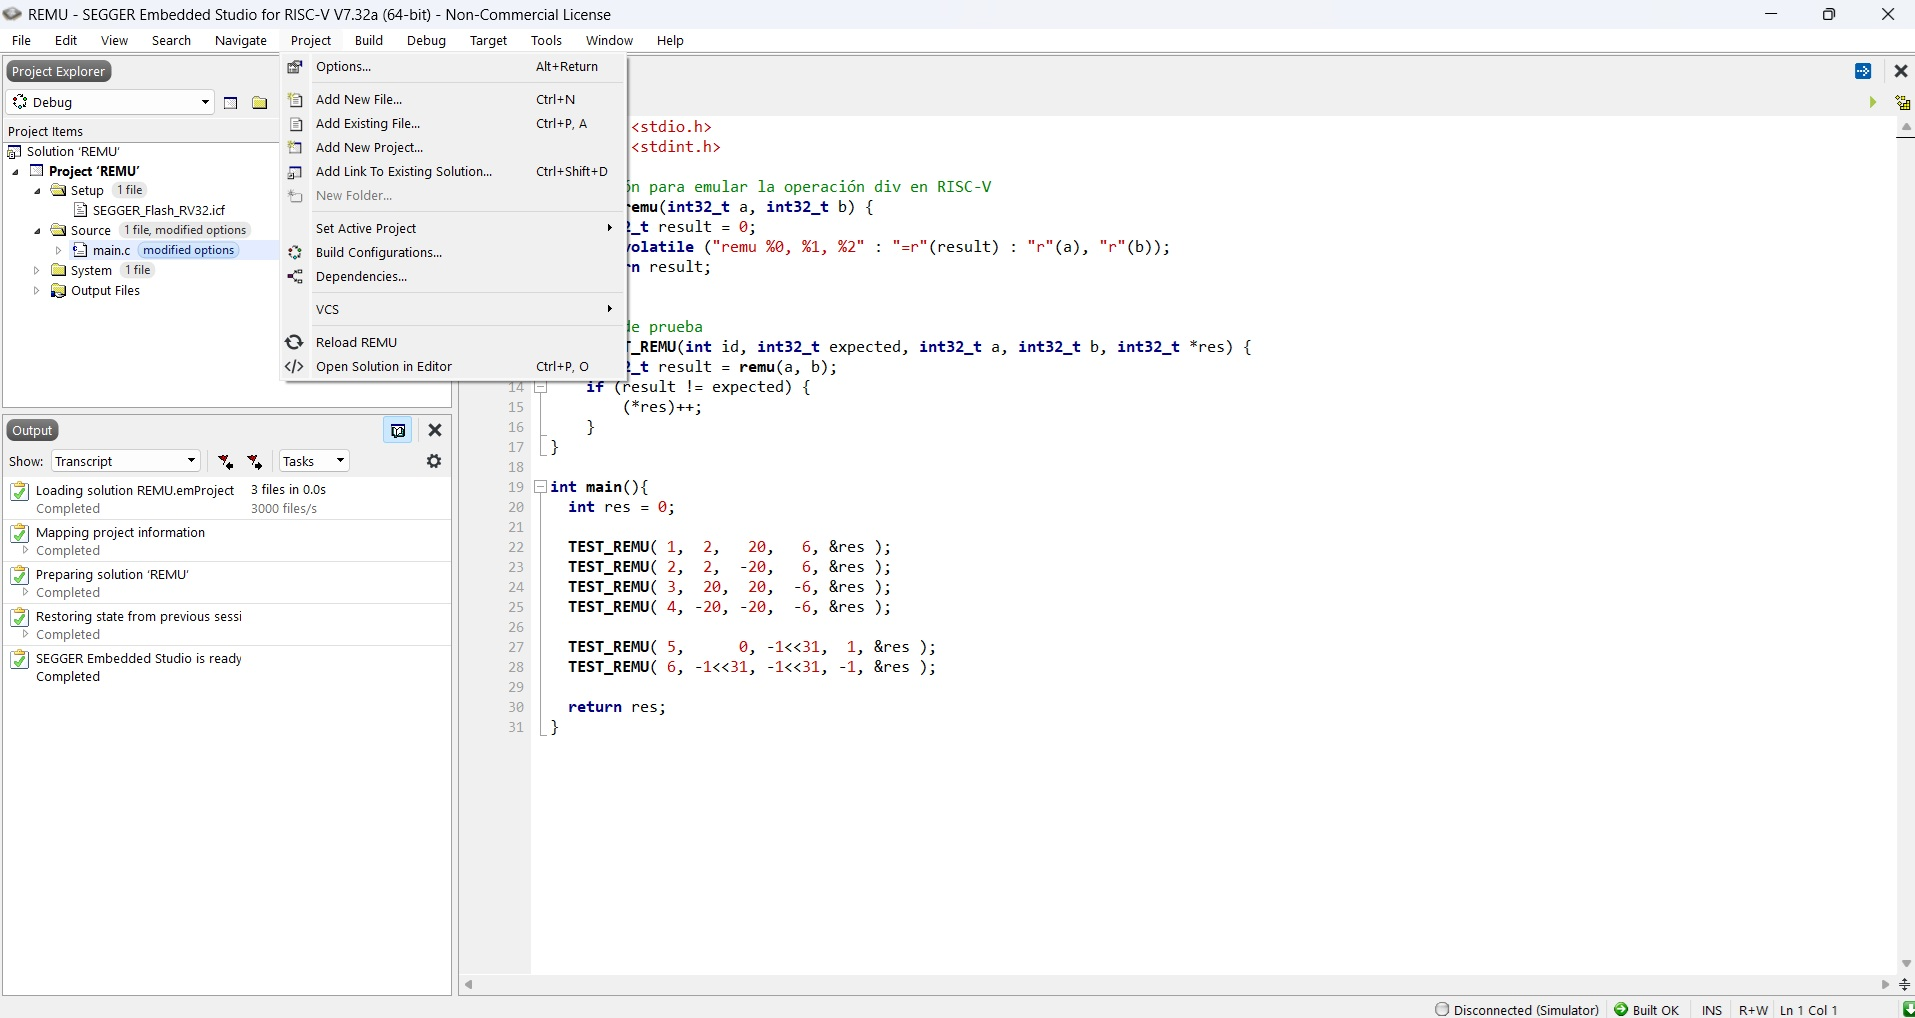
\includegraphics[width=\textwidth]{imaxes/Cap_1.jpg}
  \caption{Opcións do proxecto}
  \label{fig:cap1}
\end{figure}

\begin{figure}[hp!]
  \centering
  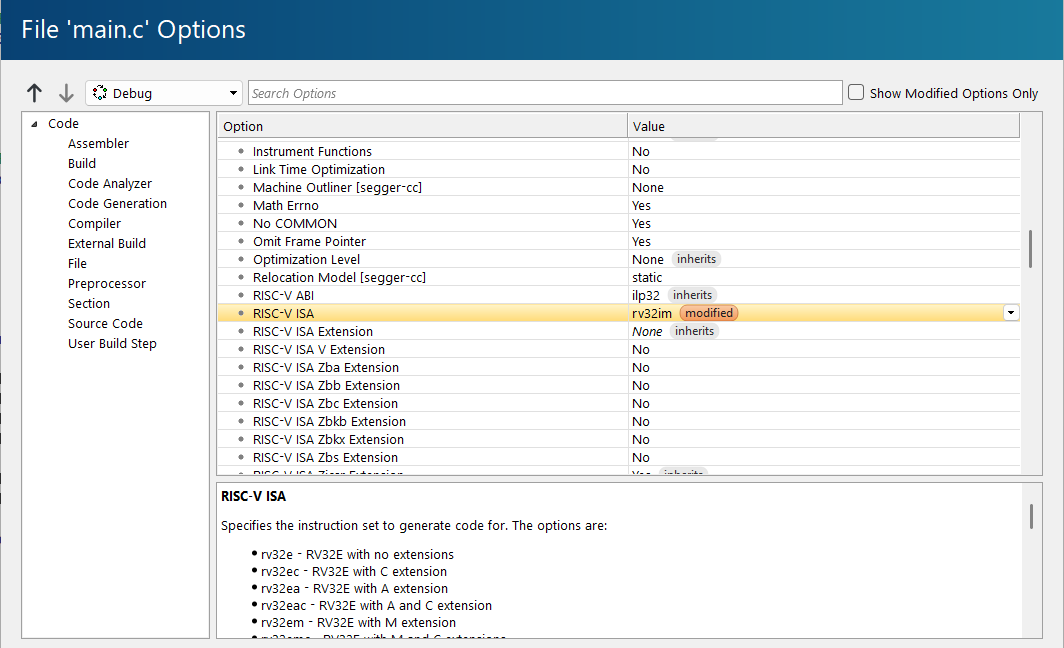
\includegraphics[width=\textwidth]{imaxes/Cap_2.png}
  \caption{Elección da extensión correcta}
  \label{fig:cap2}
\end{figure}

 Unha vez feito isto,  Build -> Build Solution, como mostra a captura \ref{fig:compilar}. Agora na carpeta Output Files, están varios arquivos, entre eles o executable con extensión .elf. É posible executar e depurar o código dentro do propio Segger, podendo así comprobar se o test está correcto de forma rápida (ver \ref{fig:cap3}).

\begin{figure}[hp!]
  \centering
  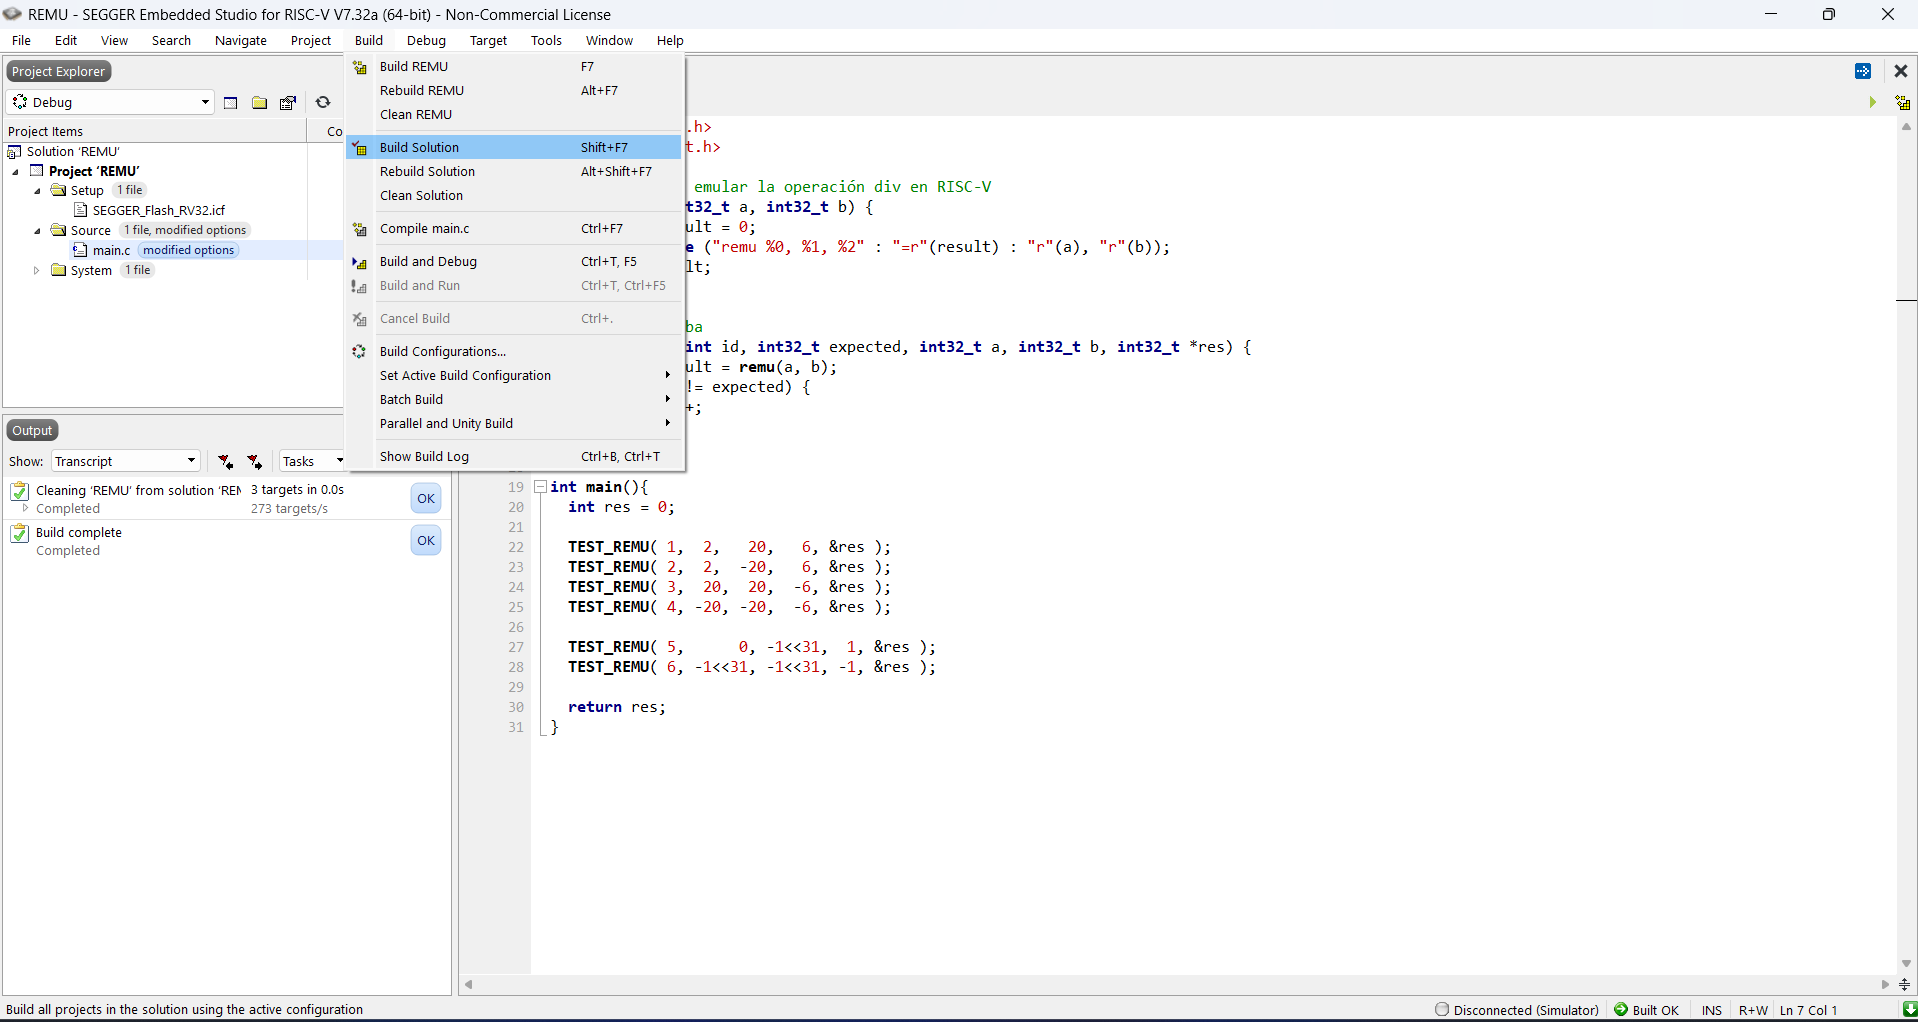
\includegraphics[width=\textwidth]{imaxes/Cap_3_Comp.png}
  \caption{Compilación do proxecto}
  \label{fig:compilar}
\end{figure}

\begin{figure}[hp!]
  \centering
  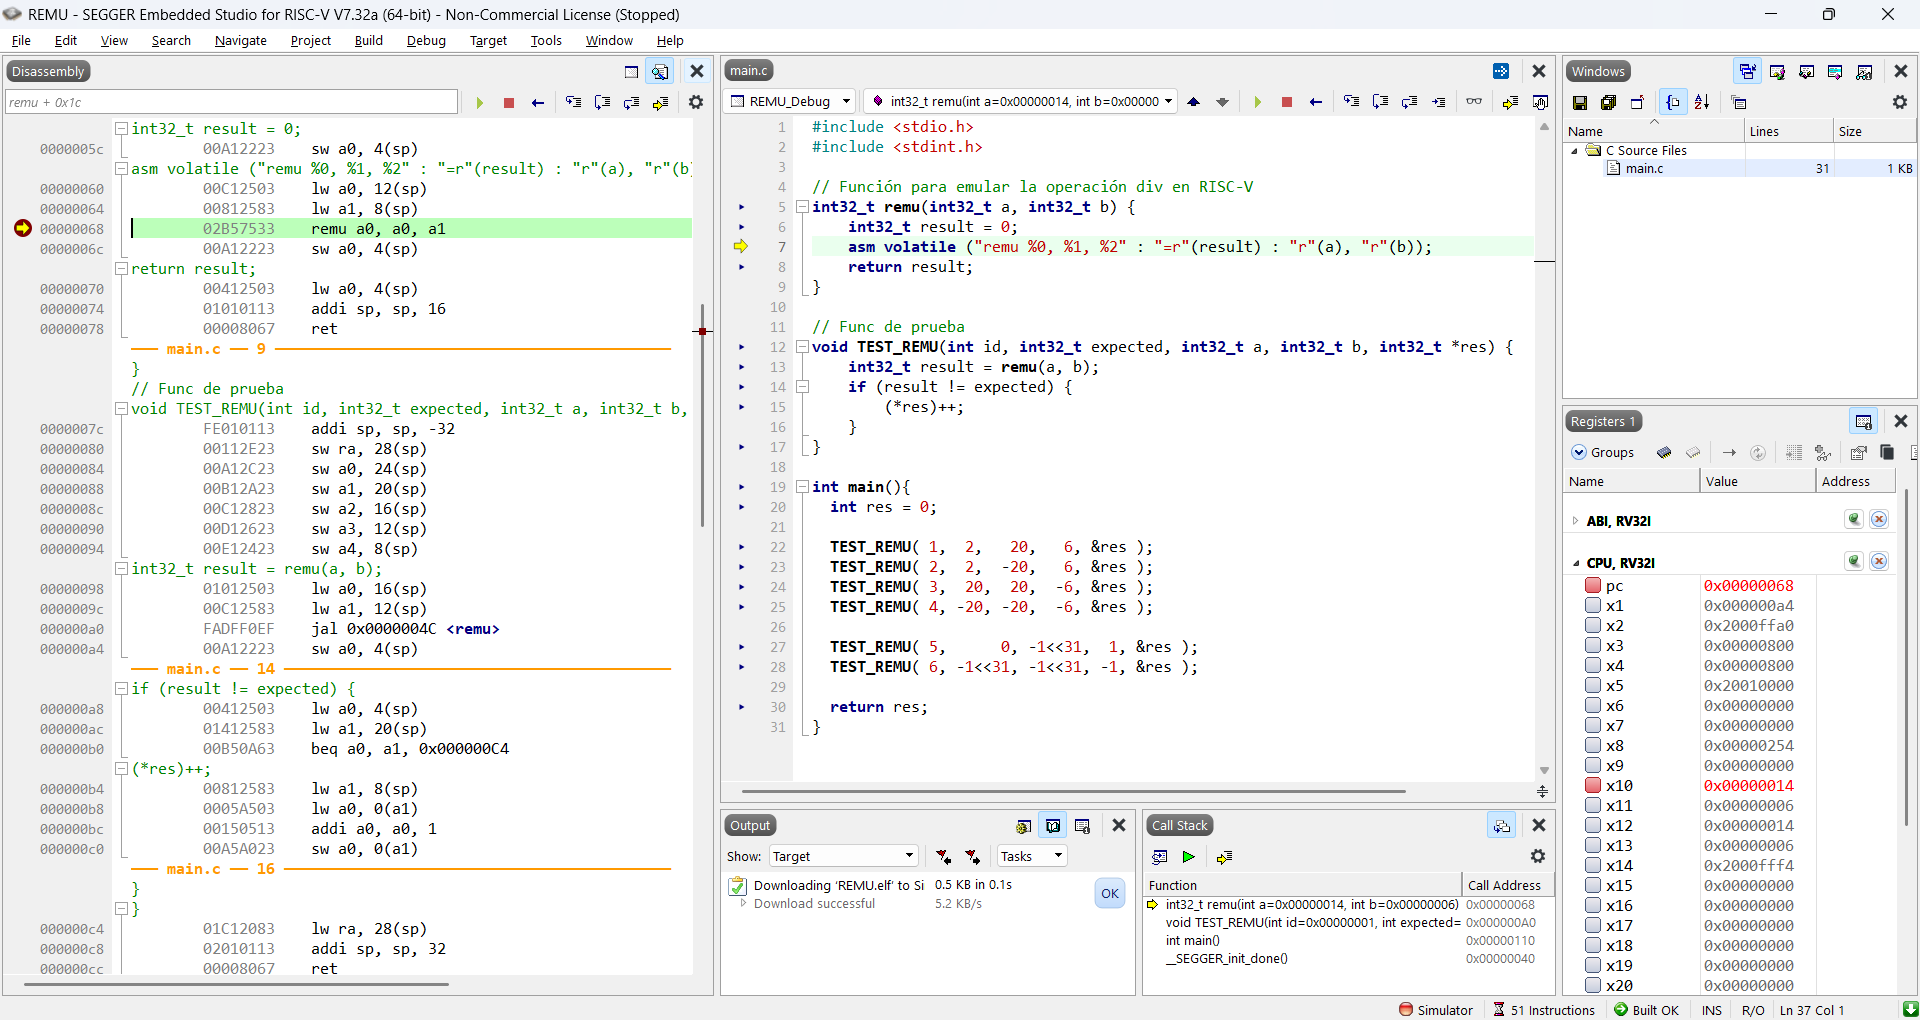
\includegraphics[width=\textwidth]{imaxes/Cap_4_Debug.png}
  \caption{Captura coas opcións de depuración de Segger}
  \label{fig:cap3}
\end{figure}

Para o axuste de parámetros debemos ir á Visual Studio 2022, no ficheiro config.h, aparecen definidas constantes para a latencia de instrucións, co nomes que seguen o formato LatencyNomeInstrución, por exemplo LatencyMul, como se ve na captura \ref{fig:parametros}. Finalmente, abrirase unha pantalla onde se mostrará que módulos están compilados, o tempo, o número de ciclos e o número de instrucións que levou o test. Importante revisar se o resultado é correcto, para isto tal e como se mostra na \ref{fig:resultados} imprímese o valor do rexistro x10, onde se almacena un 0 se o resultado é o esperado ou 1 se hai algún erro.

\begin{figure}[hp!]
  \centering
  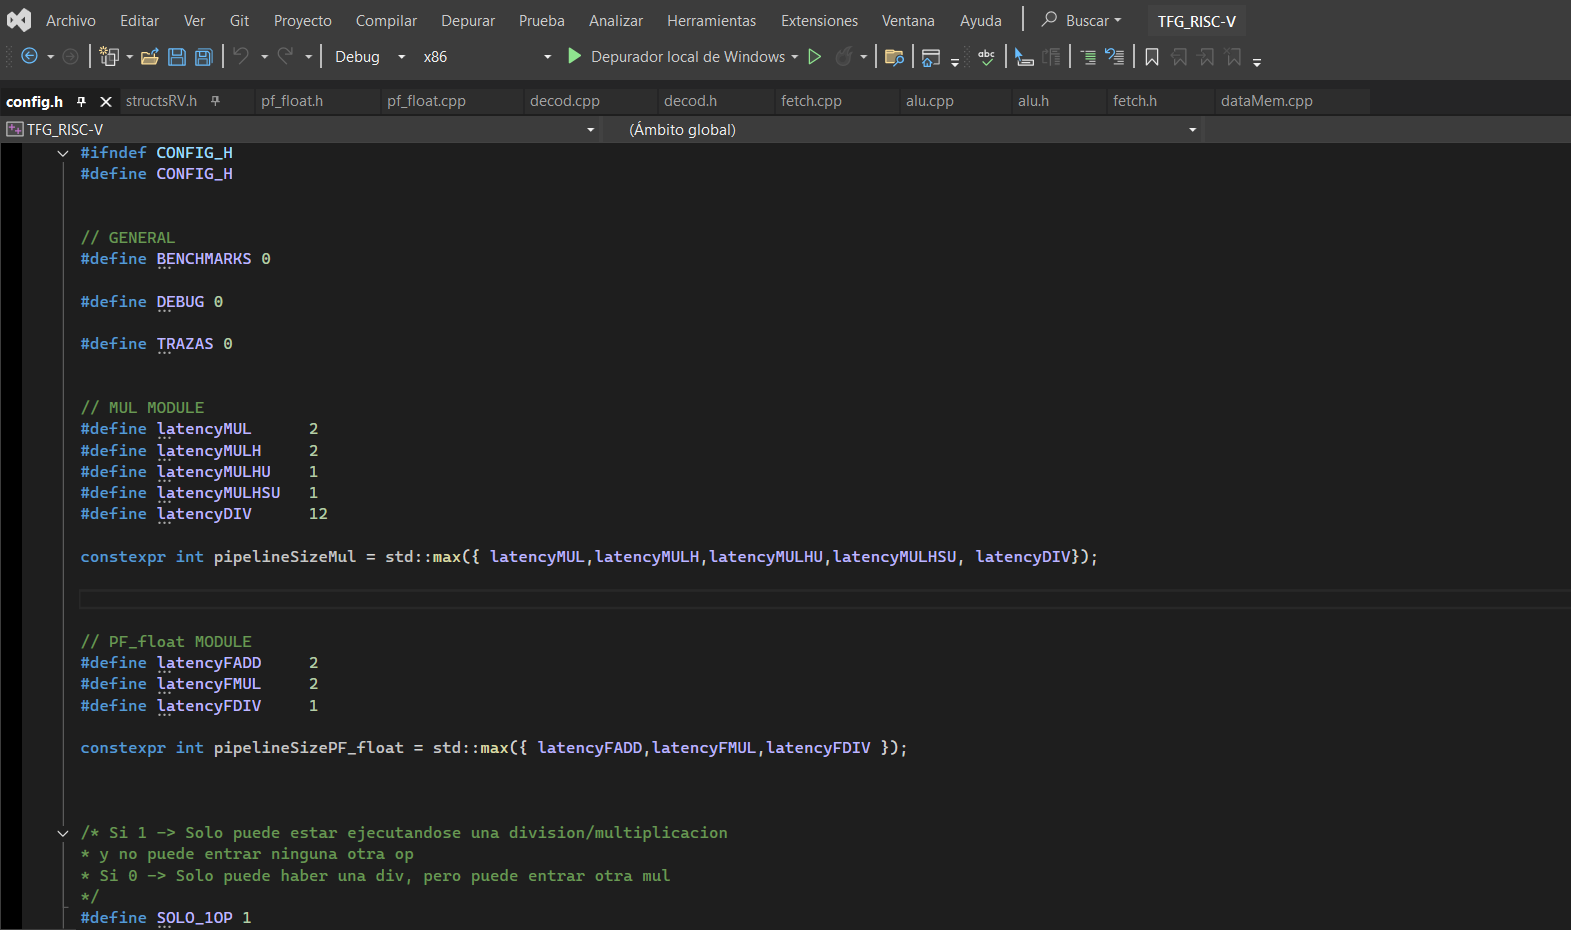
\includegraphics[width=\textwidth]{imaxes/Cap_5_Config.png}
  \caption{Cambio de parámetros en Config.h}
  \label{fig:parametros}
\end{figure}

\begin{figure}[hp!]
  \centering
  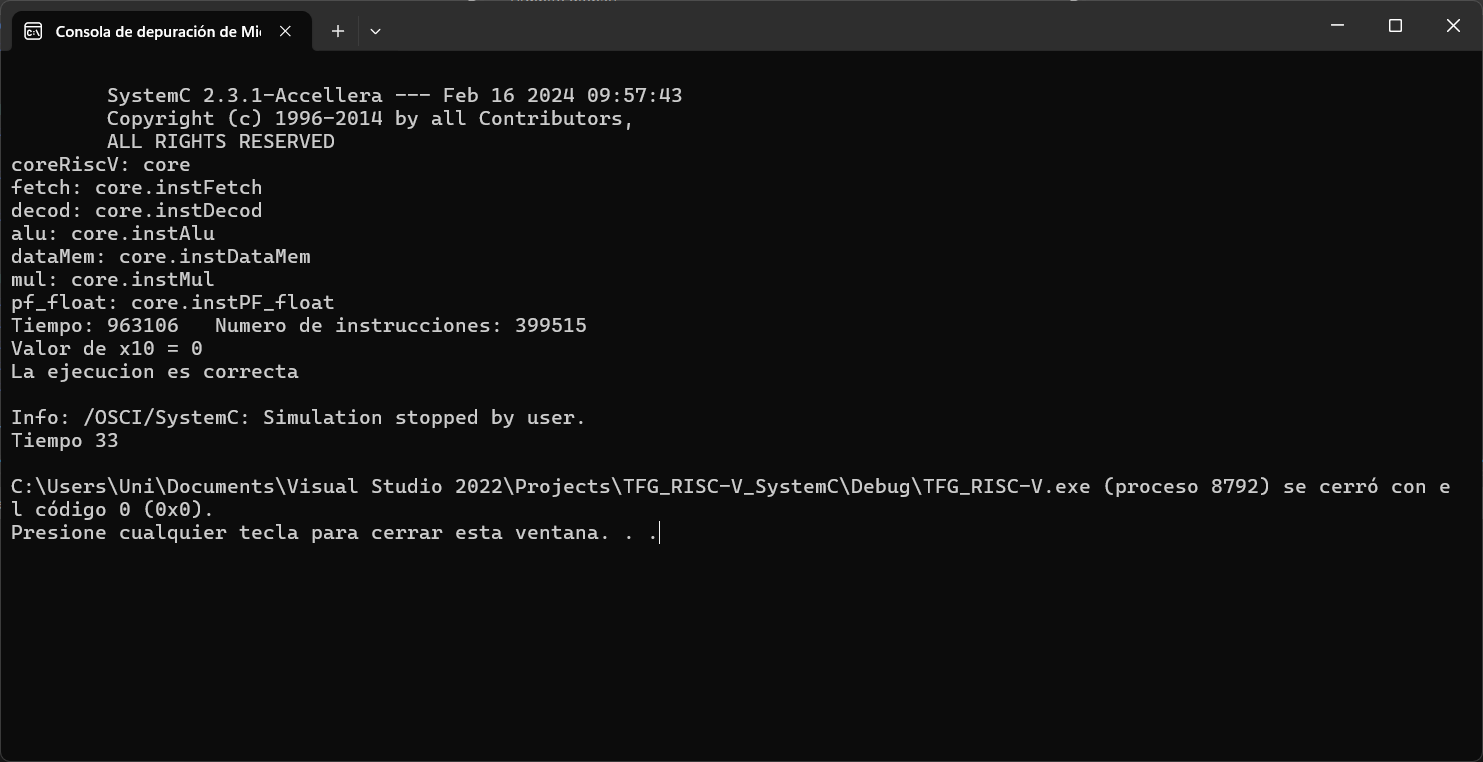
\includegraphics[width=\textwidth]{imaxes/Cap_res_final.png}
  \caption{Resultados tras executar o benchmark SPMV}
  \label{fig:resultados}
\end{figure}



\chapter{Conclusións}
\label{chap:conclusions}

\lettrine{D}{erradeiro} capítulo da memoria, onde se presentará a
situación final do traballo, as leccións aprendidas, a relación coas competencias da titulación en xeral e a mención en particular,
posibles liñas futuras,\dots

\section{Resultados}\label{chap:resultados}
Tras finalizar o proxecto, pódese garantir que engadir novas extensións coas súas correspondentes novas instrucións non comprometen o traballo anterior. O funcionamento do resto de módulos segue sendo correcto, o rendemento non se viu deteriorado en ningún momento.

Por outra parte, a posibilidade de modificar as latencias dalgunhas instrucións grazas á parametrización engadida, mostra como cambia o rendemento no conxunto dun programa. Por exemplo, á hora de executar o benchmark SPMV para que realice multiplicación de enteiros, obtemos resultados moi interesantes segundo as latencias. Como vemos na táboa \ref{tab:rendemento_spmv}, 

\begin{table}[hp!]
    \centering
    \rowcolors{2}{white}{udcgray!25}
    \begin{tabular}{c|c|c}
    \rowcolor{udcpink!25}
    \textbf{Modificacións realizadas} & \textbf{Número de instrucións}  & \textbf{Tempo} 
    \\\hline
    \textit{SPMV base} & a & a \\
    \textit{Latencia de mul = 5} & a & b\\
    \textit{Latencia de mul = 10} & a & b\\
    \textit{Latencia de mulh = 5} & a & b\\
    \textit{Latencia de mul = 5 e mulh = 5} & a & b\\
    \end{tabular}
    \caption{Rendemento do benchmarks SPMV segundo as latencia de distintas operacións.}
    \label{tab:rendemento_spmv}
\end{table}

Finalmente, destacar que a velocidade de simulación deste proxecto en comparación coa que se podería obter se VHDL ou Verilog fose empregado é moi superior.

\section{Traballo futuro}\label{chap:traballo_futuro}
Agora mesmo, o simulador inclúe todas as instrucións implementadas ata o que é conecido como extensión 'G'. Poderíanse engadir máis extensións, así como unha memoria ¿? ou incluir soporte para 64bits.




 %%%%%%%%%%%%%%%%%%%%%%%%%%%%%%%%%%%%%%%%
 % Apéndices, glosarios e bibliografía  %
 %%%%%%%%%%%%%%%%%%%%%%%%%%%%%%%%%%%%%%%%

 \appendix
 \appendixpage
 \appendix
\chapter{Material adicional}
\label{chap:adicional}

\lettrine{E}{ste} capítulo ten formato de apéndice, inclúe material adicional que non ten cabida no corpo principal do documento, como código de tests ou exemplos de módulos.

\section{Exemplo de código de probas}
\label{cod_test}

\begin{lstlisting}[language=C]
#include <stdio.h>
#include <stdint.h>

// Función para emular la operación remu en RISC-V
int32_t remu(int32_t a, int32_t b) {
    int32_t result = 0;
    asm volatile ("remu %0, %1, %2" : "=r"(result) : "r"(a), "r"(b));
    return result;
}

// Funcion de prueba
void TEST_REMU(int id, int32_t expected, int32_t a, int32_t b, int32_t *res) {
    int32_t result = remu(a, b); 
    if (result != expected) {
        (*res)++;
    }
}

int main(){
  int res = 0;

  TEST_REMU( 1,  2,   20,   6, &res );
  TEST_REMU( 2,  2,  -20,   6, &res );
  TEST_REMU( 3,  20,  20,  -6, &res );
  TEST_REMU( 4, -20, -20,  -6, &res );

  TEST_REMU( 5,      0, -1<<31,  1, &res );
  TEST_REMU( 6, -1<<31, -1<<31, -1, &res );

  return res;
}
\end{lstlisting}

\section{Módulo de multiplicación}
\label{mul_module}
A continuación móstrase o código do módulo de multiplicación, composto polo ficheiro de cabeceira e o correspondente corpo. 

\begin{lstlisting}[language=C++]
#ifndef MUL_H
#define MUL_H

#include "systemc.h"
#include "structsRV.h"
#include "config.h"
#include "auxFuncs.h"


SC_MODULE(mul) {
public:

	sc_in <bool> clk, rst;
	sc_in <instruction> I;

	// Hazard detection from Decod
	sc_in <sc_uint<5>> rs1In, rs2In;
	sc_out <bool> hzrdRs1Out, hzrdRs2Out;

	sc_out <bool> readyFenceMulOut;

	sc_out <instruction> instOut;


	void multiplication();

	void hazardDetection();

	SC_CTOR(mul) {
		cout << "mul: " << name() << endl;

		// NOP
		INST = createNOP();

		SC_METHOD(multiplication);
		sensitive << clk.pos();

		SC_METHOD(hazardDetection);
		sensitive << rs1In << rs2In << fire;

		fire.write(true);

	}

private:

	instruction INST;
	sc_signal <bool> fire;

	instruction pipeline[pipelineSizeMul];

	bool pipelineFull = false;
	bool flagDiv = false;

};

#define MUL 16
#define MULH 17
#define MULHSU 18
#define MULHU 19
#define DIV 20
#define DIVU 21
#define REM 22
#define REMU 23

#endif
\end{lstlisting}

\begin{lstlisting}[language=C++]
#include "mul.h"
#include "alu.h"


// COMPLETELY SEGMENTED
void mul::multiplication() { 

	sc_int <32> A, B, res;
	sc_uint <5> opCode;
	short target;
	double tiempo;

	tiempo = sc_time_stamp().to_double() / 1000.0;

	if (rst.read()) {

		// NOP
		INST = createNOP();
		instOut.write(INST); 

		// empty pipeline
		for (int i = 0; i < pipelineSizeMul; i++) {
			pipeline[i] = createNOP();
		}


	} else {
		
		// Get data
		INST = I.read();

		A = INST.opA;
		B = INST.opB;
		target = INST.rd;
		opCode = INST.aluOp;

		// Independant pipeline for each instruction 
		int cyclesInPipeline = 0;
		instruction output = pipeline[0];

		for (int i = 0; i < pipelineSizeMul - 1; i++) {

			cyclesInPipeline = pipelineSizeMul - i;

			if (pipeline[i].wReg && getLatencyOp(pipeline[i].aluOp,pipeline[i].target) <= cyclesInPipeline) {

				output = pipeline[i];
				pipeline[i] = createNOP();

				// Div in output
				if (pipeline[i].aluOp == DIV || pipeline[i].aluOp == DIVU || 
					pipeline[i].aluOp == REM || pipeline[i].aluOp == REMU ) {
					flagDiv = false;
					pipelineFull = false;
				}
				break;
			}
		}

		if (output.aluOp != 0) {
			pipelineFull = false;
		}

		instOut.write(output);

		// Loop to shift pipeline content
		// Pos 0: exit
		// Pos latencyMUL-1: newElement
		for (int i = 0; i < pipelineSizeMul - 1; i++) {
			pipeline[i] = pipeline[i + 1];
		}

		sc_int<64> tmp = 0;

		// Operate
		switch (opCode)
		{
		case MUL: 
			tmp = ((sc_int<32>)A) * ((sc_int<32>)B);
			INST.aluOut = INST.dataOut = tmp(31,0);
			strcpy(INST.desc, "mul");
			break;

		case MULH: 
			tmp = ((sc_int<32>)A) * ((sc_int<32>)B);
			INST.aluOut = INST.dataOut = tmp(63,32);
			strcpy(INST.desc, "mulh");
			break;

		case MULHU:
			tmp = ((sc_uint<32>)A) * ((sc_uint<32>)B);
			INST.aluOut = INST.dataOut = tmp(63, 32);
			strcpy(INST.desc, "mulhu");
			break;

		case MULHSU:
			tmp = ((sc_int<32>)A) * ((sc_uint<32>)B);
			INST.aluOut = INST.dataOut = tmp(63, 32);
			strcpy(INST.desc, "mulhsu");
			break;

		case DIV:
			if (B == 0) {
				cerr << "Divider can't be 0 " << endl;
			}
			INST.aluOut = INST.dataOut = ((sc_int<32>)A) / ((sc_int<32>)B);
			strcpy(INST.desc, "div");
			flagDiv = true;
			break;

		case DIVU:
			if (B == 0) {
				cerr << "Divider can't be 0 " << endl;
			}
			INST.aluOut = INST.dataOut =((sc_uint<32>)A) / ((sc_uint<32>)B);
			strcpy(INST.desc, "divu");
			flagDiv = true;
			break;

		case REM:
			if (B == 0) {
				cerr << "Divider can't be 0 " << endl;
			}
			INST.aluOut = INST.dataOut = ((sc_int<32>)A) % ((sc_int<32>)B);
			strcpy(INST.desc, "rem");
			flagDiv = true;
			break;

		case REMU:
			if (B == 0) {
				cerr << "Divider can't be 0 " << endl;
			}
			INST.aluOut = INST.dataOut =  ((sc_uint<32>)A) % ((sc_uint<32>)B);
			strcpy(INST.desc, "remu");
			flagDiv = true;
			break;

		default:
			INST = createNOP();
			break;
		}

		// New instruction
		pipeline[pipelineSizeMul - 1] = INST;

	} 
	fire.write(!fire.read());
}

void mul::hazardDetection() {

	int rs1 = rs1In.read();
	int rs2 = rs2In.read();


	bool aux1 = false, 
		 aux2 = false;

	int cont = 0;
	bool emptyPipeline = false;

	// Prevents RAW
	for (int i = 0; i < pipelineSizeMul; i++) {

		if (pipeline[i].wReg) {

			if (rs1 == pipeline[i].rd) {
				aux1 = true;
			}

			if (rs2 == pipeline[i].rd) {
				aux2 = true;
			}
		}
		else {
			cont++;
		}
	}

	if (instOut.read().wReg) {

		if (rs1 == instOut.read().rd) {
			aux1 = true;
		}

		if (rs2 == instOut.read().rd) {
			aux2 = true;
		}
	}
	else {
		emptyPipeline = true;
	}

#if SOLO_1OP

	if (I.read().wReg) {
		int opCode = I.read().aluOp;

		if (isMulModuleOp(opCode)) {
			aux1 = aux2 = true;
			pipelineFull = true;
		}
		else if (!pipelineFull) {
			aux1 = aux2 = false;
		}
	}
	else {
		emptyPipeline = emptyPipeline && true;
	}
	
	
#else

	if (I.read().wReg) {
		int opCode = I.read().aluOp;

		if (flagDiv && isMulModuleOp(opCode)) {
			if (opCode == DIV || opCode == DIVU || opCode == REM || opCode == REMU) {
				aux1 = aux2 = true;
			}
			else {
				aux1 = aux2 = false;
			}
		}
	}
	else {
		aux1 = aux2 = false;
		emptyPipeline = emptyPipeline && true;
	}
#endif
	
	if (cont == pipelineSizeMul && emptyPipeline) {
		readyFenceMulOut.write(true);
	}
	else {
		readyFenceMulOut.write(false);
	}

	hzrdRs1Out.write(aux1);
	hzrdRs2Out.write(aux2);
}
\end{lstlisting}

%\include{anexos/...}

 \printglossary[type=\acronymtype,title=\nomeglosarioacronimos]
 \printglossary[title=\nomeglosariotermos]

 \bibliographystyle{IEEEtranN}
 \bibliography{\bibconfig,bibliografia/bibliografia}
 \clearpage
 
\end{document}

%%%%%%%%%%%%%%%%%%%%%%%%%%%%%%%%%%%%%%%%%%%%%%%%%%%%%%%%%%%%%%%%%%%%%%%%%%%%%%%%
